\documentclass[11pt,a4paper]{article}
\usepackage[utf8]{inputenc}
\usepackage[T1]{fontenc}
\usepackage{amsmath,amssymb}
\usepackage{graphicx}
\usepackage{booktabs}
\usepackage{hyperref}
\usepackage[margin=2.2cm]{geometry}
\usepackage{caption}
\usepackage{subcaption}
\usepackage{xcolor}
\usepackage{float}

\definecolor{robust}{HTML}{E74C3C}
\definecolor{blended}{HTML}{2ECC71}

\title{\textbf{Predicting Augmentation Transforms\\Makes Models More Robust}}
\author{}
\date{}

\begin{document}
\maketitle

\begin{abstract}
We show that adding a lightweight auxiliary task---predicting which data augmentation transform was applied to each training image---substantially improves model robustness to image corruptions. The auxiliary loss contributes at most 1\% to the total training objective, yet it reduces the average accuracy drop under corruption by \textbf{2--3$\times$} compared to standard robust training (data augmentation alone). This improvement holds consistently across four backbone architectures (ResNet18, VGG16, VGG19, Vision Transformer) on CIFAR-10 and generalizes to out-of-distribution corruptions never seen during training.
\end{abstract}

%---------------------------------------------------------------------
\section{Method}

\subsection{Continuous Transforms}

Both training strategies use the same pool of continuous image transforms, parameterized by a severity $s \in [0, 1]$:

\begin{itemize}
    \item \textbf{Gaussian noise}: additive noise with $\sigma = 0.5 \cdot s$
    \item \textbf{Rotation}: angle sampled from $[-360s, +360s]$ degrees
    \item \textbf{Affine}: translation $\in [-0.1s, +0.1s]$ (image fraction), shear $\in [-15s, +15s]$ degrees
    \item \textbf{No transform}: identity (image unchanged)
\end{itemize}

\subsection{Robust Training (Baseline)}

The Robust model is a \textbf{plain classifier} with a single output head. During training, each image has a 50\% probability of being augmented with a random transform (excluding \texttt{no\_transform}) at severity $s \sim \mathcal{U}[0,\, 0.5]$. The loss is standard cross-entropy:
\begin{equation}
    \mathcal{L}_{\text{robust}} = \text{CE}(\hat{y},\; y)
\end{equation}

\subsection{Blended Training (Proposed)}

The Blended model augments the backbone with four lightweight auxiliary heads and a feature fusion module:

\begin{enumerate}
    \item \textbf{Transform type head}: predicts which of the 4 transforms was applied ($D \to 4$)
    \item \textbf{Rotation head}: predicts the rotation angle ($D \to 1$)
    \item \textbf{Noise head}: predicts the noise level ($D \to 1$)
    \item \textbf{Affine head}: predicts affine parameters ($D \to 4$)
\end{enumerate}

The auxiliary predictions (10 values) are concatenated with the backbone features ($D$ dimensions) and passed through a two-layer fusion MLP ($D{+}10 \to D$). A \textbf{residual connection} adds the fused features back to the original backbone features, ensuring the auxiliary pathway can only enhance the representation:
\begin{equation}
    \mathbf{h}_{\text{enhanced}} = \mathbf{h}_{\text{backbone}} + \text{FusionMLP}\big([\mathbf{h}_{\text{backbone}},\; \hat{\mathbf{t}}]\big)
\end{equation}
where $\hat{\mathbf{t}}$ denotes the concatenated transform predictions.

During training, \textbf{every} image is transformed with a random transform (including \texttt{no\_transform}) at severity $s \sim \mathcal{U}[0,\, 1.0]$. The loss couples classification and transform prediction:
\begin{equation}
    \mathcal{L}_{\text{blended}} = \mathcal{L}_{\text{cls}} + 0.01 \cdot \mathcal{L}_{\text{cls}} \cdot \sigma\!\big(\mathcal{L}_{\text{transform}}\big)
\end{equation}
where $\mathcal{L}_{\text{cls}} = \text{CE}(\hat{y}, y)$, $\mathcal{L}_{\text{transform}} = \text{CE}(\hat{t}, t)$ is the transform type prediction loss, and $\sigma$ is the sigmoid function. Since $\sigma(\cdot) \in [0, 1]$, the auxiliary term increases the classification loss by \textbf{at most 1\%}.

\subsection{Training Differences}

\begin{table}[H]
\centering
\caption{Comparison of Robust and Blended training configurations.}
\label{tab:training_diff}
\begin{tabular}{lcc}
\toprule
\textbf{Aspect} & \textbf{Robust} & \textbf{Blended} \\
\midrule
Architecture & Plain classifier & + 4 aux heads + fusion MLP \\
Transform probability & 50\% per image & 100\% per image \\
Severity range & $\mathcal{U}[0,\, 0.5]$ & $\mathcal{U}[0,\, 1.0]$ \\
Transform pool & 3 (excl.\ no\_transform) & 4 (incl.\ no\_transform) \\
Loss & $\text{CE}$ & $\text{CE} + 0.01 \cdot \text{CE} \cdot \sigma(\text{CE}_t)$ \\
Effective aux weight & --- & $\leq 0.01$ \\
\bottomrule
\end{tabular}
\end{table}

%---------------------------------------------------------------------
\section{Evaluation}

Models are evaluated on: (1)~corrupted data at severities $\{0.25, 0.5, 0.75, 1.0\}$ with transforms sampled uniformly from $\{$no\_transform, gaussian\_noise, rotation, affine$\}$; and (2)~out-of-distribution (OOD) data with 10 extreme corruptions never seen during training (color inversion, pixelation, extreme blur, channel shuffle, posterization, solarization, JPEG compression, random masking, extreme noise, extreme rotation).

%---------------------------------------------------------------------
\section{Results}

\subsection{Overall Accuracy}

\begin{table}[H]
\centering
\caption{Accuracy at increasing corruption severity and OOD. \textbf{Bold} = better in each pair. Avg Drop = mean accuracy decrease from clean across $s \in \{0.25, 0.5, 0.75, 1.0\}$.}
\label{tab:overall}
\begin{tabular}{llccccccc}
\toprule
\textbf{Backbone} & \textbf{Model} & \textbf{Clean} & \textbf{S=0.25} & \textbf{S=0.5} & \textbf{S=0.75} & \textbf{S=1.0} & \textbf{Avg Drop} & \textbf{OOD} \\
\midrule
\multirow{2}{*}{ResNet18}
 & Robust  & 66.5 & 51.1 & 43.9 & 42.2 & 41.4 & 0.219 & 34.1 \\
 & \textbf{Blended} & \textbf{83.1} & \textbf{76.9} & \textbf{72.8} & \textbf{70.2} & \textbf{68.5} & \textbf{0.111} & \textbf{46.6} \\
\midrule
\multirow{2}{*}{VGG16}
 & Robust  & \textbf{85.7} & 69.8 & 57.0 & 54.5 & 54.6 & 0.267 & 43.5 \\
 & \textbf{Blended} & 82.7 & \textbf{76.2} & \textbf{72.8} & \textbf{70.1} & \textbf{67.5} & \textbf{0.110} & \textbf{44.7} \\
\midrule
\multirow{2}{*}{VGG19}
 & Robust  & \textbf{88.6} & 73.7 & 61.1 & 57.9 & 57.6 & 0.260 & \textbf{46.9} \\
 & \textbf{Blended} & 81.6 & \textbf{75.1} & \textbf{72.2} & \textbf{68.3} & \textbf{66.5} & \textbf{0.111} & 44.8 \\
\midrule
\multirow{2}{*}{ViT}
 & Robust  & \textbf{79.5} & 64.1 & 52.7 & 50.1 & 49.9 & 0.253 & \textbf{38.5} \\
 & \textbf{Blended} & 70.3 & \textbf{65.4} & \textbf{62.3} & \textbf{59.7} & \textbf{58.2} & \textbf{0.089} & 37.8 \\
\bottomrule
\end{tabular}
\end{table}

\subsection{Per-Transform Accuracy at Maximum Severity ($s = 1.0$)}

\begin{table}[H]
\centering
\caption{Accuracy under each transform type at $s = 1.0$. \textbf{Bold} = better.}
\label{tab:per_transform}
\begin{tabular}{llccc}
\toprule
\textbf{Backbone} & \textbf{Model} & \textbf{Gaussian Noise} & \textbf{Rotation} & \textbf{Affine} \\
\midrule
\multirow{2}{*}{ResNet18}
 & Robust  & 10.0 & 32.9 & 55.8 \\
 & \textbf{Blended} & \textbf{52.5} & \textbf{61.1} & \textbf{77.4} \\
\midrule
\multirow{2}{*}{VGG16}
 & Robust  & 11.7 & 43.6 & 74.3 \\
 & \textbf{Blended} & \textbf{52.5} & \textbf{59.0} & \textbf{76.5} \\
\midrule
\multirow{2}{*}{VGG19}
 & Robust  & 10.4 & 52.2 & 79.1 \\
 & \textbf{Blended} & \textbf{50.9} & \textbf{57.2} & \textbf{76.0} \\
\midrule
\multirow{2}{*}{ViT}
 & Robust  & 10.3 & 42.3 & 68.2 \\
 & \textbf{Blended} & \textbf{41.6} & \textbf{52.6} & \textbf{66.4} \\
\bottomrule
\end{tabular}
\end{table}

\subsection{Robustness Improvement Factor}

\begin{table}[H]
\centering
\caption{Reduction in average accuracy drop (Robust $\to$ Blended).}
\label{tab:improvement}
\begin{tabular}{lccc}
\toprule
\textbf{Backbone} & \textbf{Robust Drop} & \textbf{Blended Drop} & \textbf{Improvement} \\
\midrule
ResNet18 & 0.219 & 0.111 & $\mathbf{2.0\times}$ \\
VGG16    & 0.267 & 0.110 & $\mathbf{2.4\times}$ \\
VGG19    & 0.260 & 0.111 & $\mathbf{2.3\times}$ \\
ViT      & 0.253 & 0.089 & $\mathbf{2.8\times}$ \\
\bottomrule
\end{tabular}
\end{table}

\subsection{Transform Prediction Accuracy}

\begin{table}[H]
\centering
\caption{Transform type prediction accuracy of Blended models (random baseline = 25\%).}
\label{tab:transform_pred}
\begin{tabular}{lcccc}
\toprule
\textbf{Model} & \textbf{S=0.25} & \textbf{S=0.5} & \textbf{S=0.75} & \textbf{S=1.0} \\
\midrule
ResNet18 Blended & 60.1 & 73.9 & 76.7 & 77.4 \\
VGG16 Blended    & 35.8 & 39.4 & 41.0 & 41.5 \\
VGG19 Blended    & 27.6 & 29.1 & 31.2 & 33.0 \\
ViT Blended      & 66.0 & 72.6 & 71.5 & 70.3 \\
\bottomrule
\end{tabular}
\end{table}

%---------------------------------------------------------------------
\section{Paired Comparisons}

\begin{figure}[H]
\centering
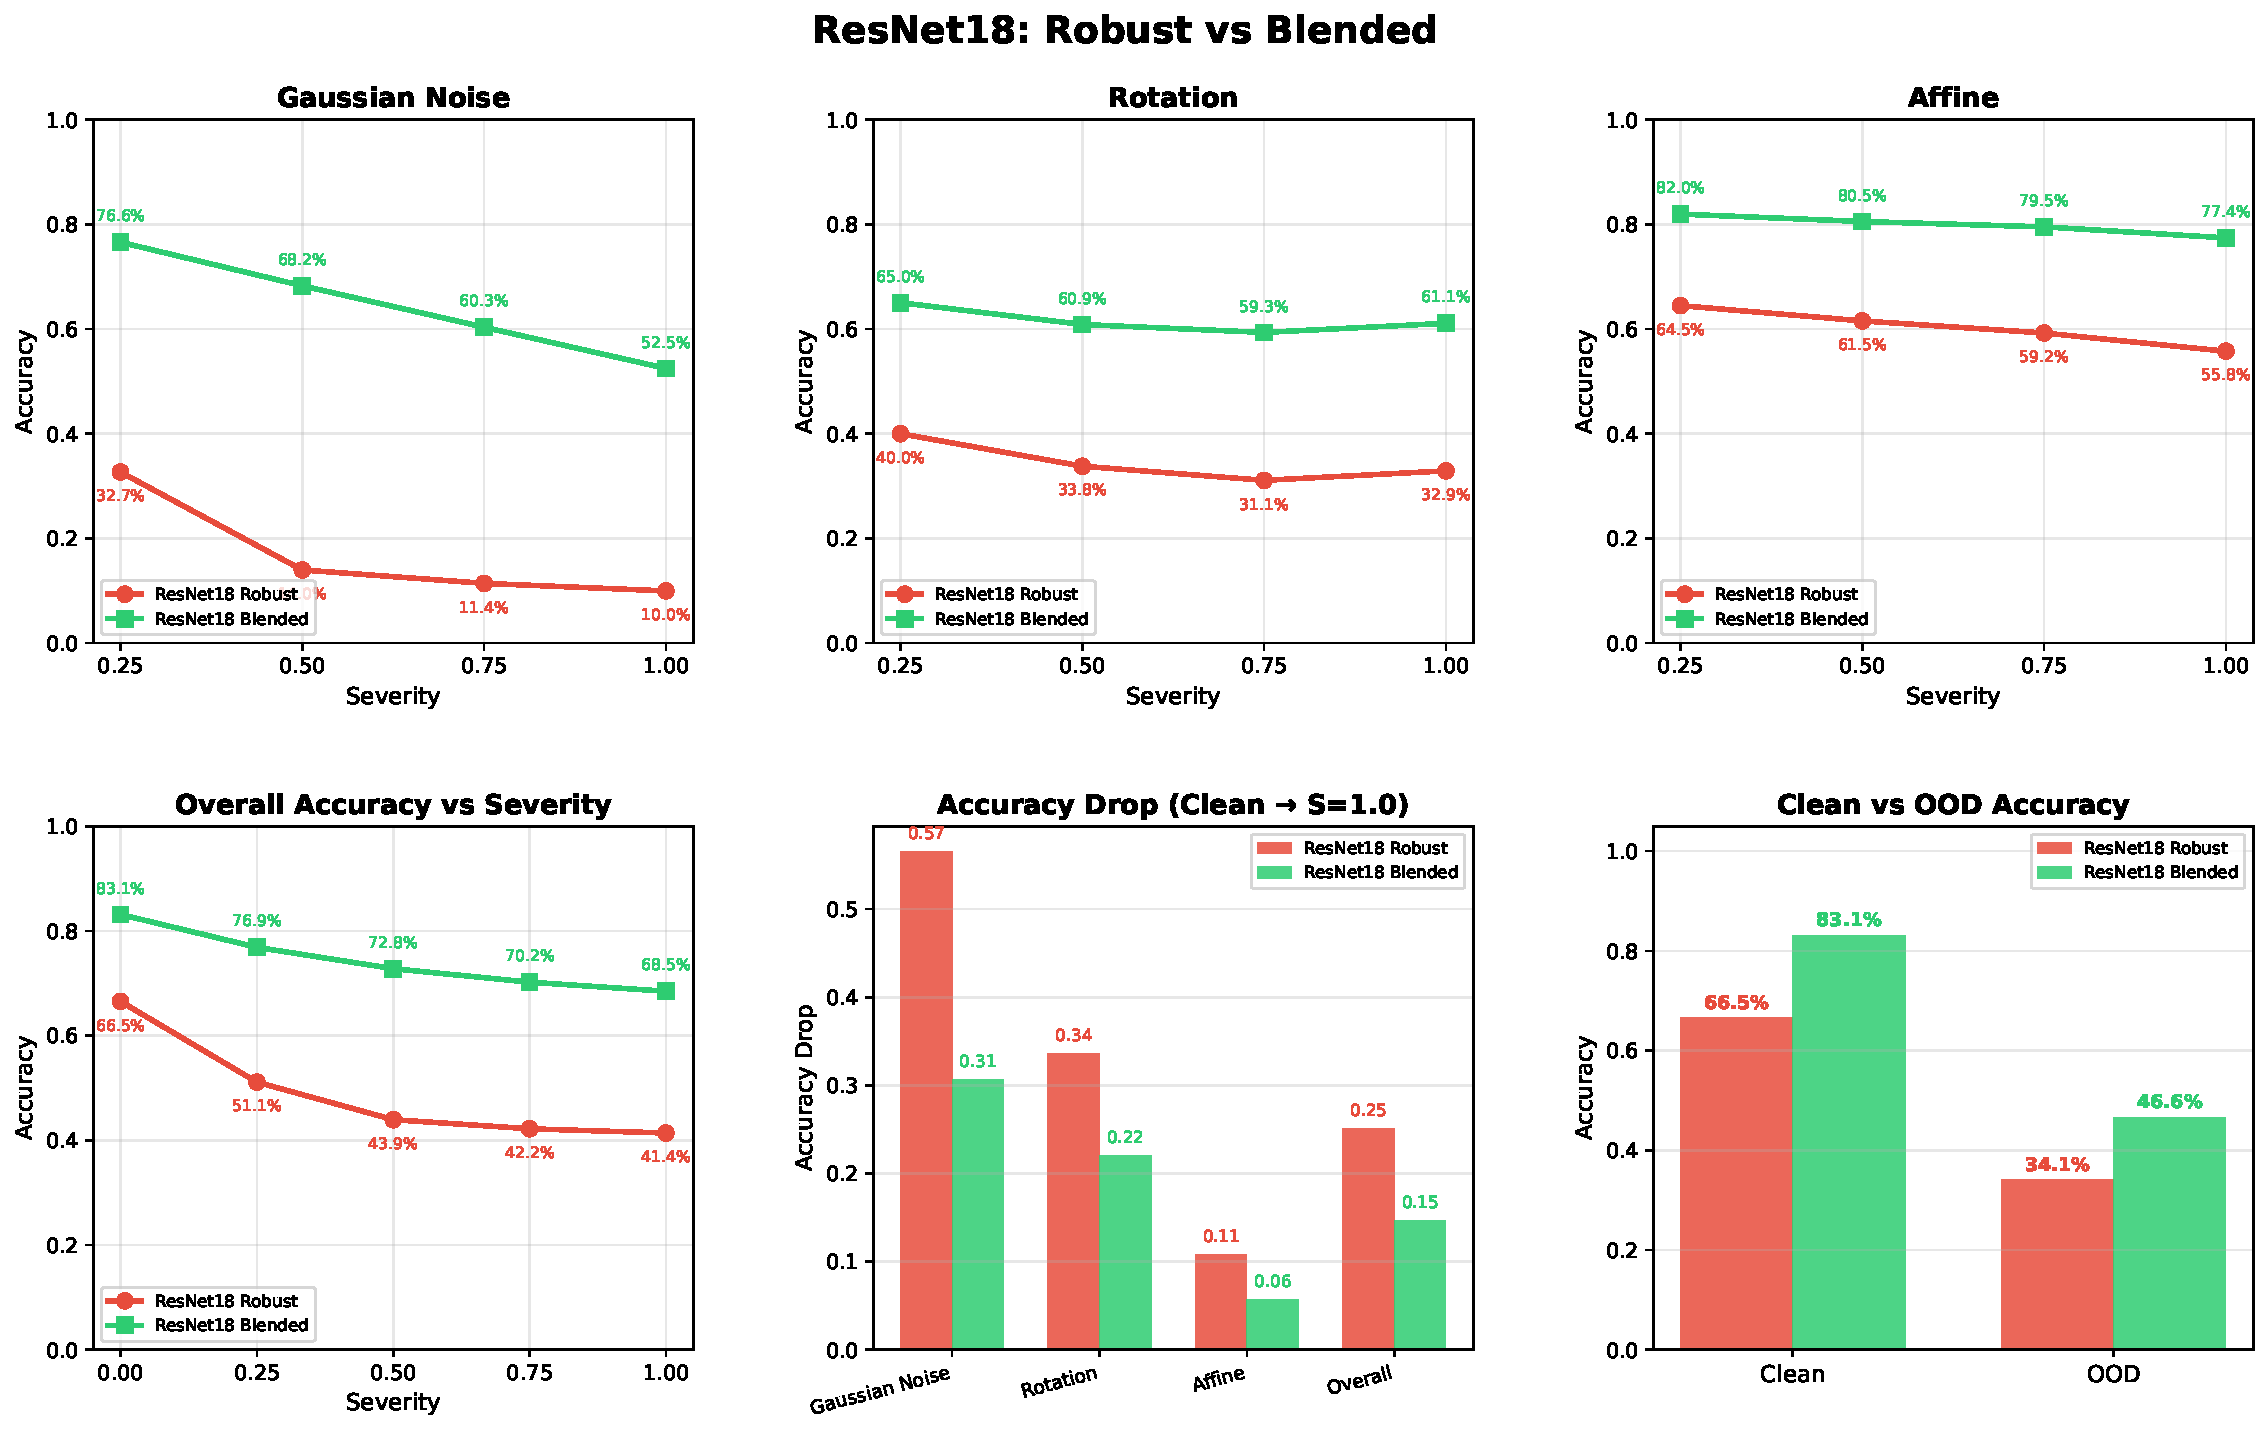
\includegraphics[width=\textwidth]{graphs/pair_resnet18_robust_vs_blended.pdf}
\caption{ResNet18: Robust vs Blended across all transforms and OOD.}
\label{fig:resnet18}
\end{figure}

\begin{figure}[H]
\centering
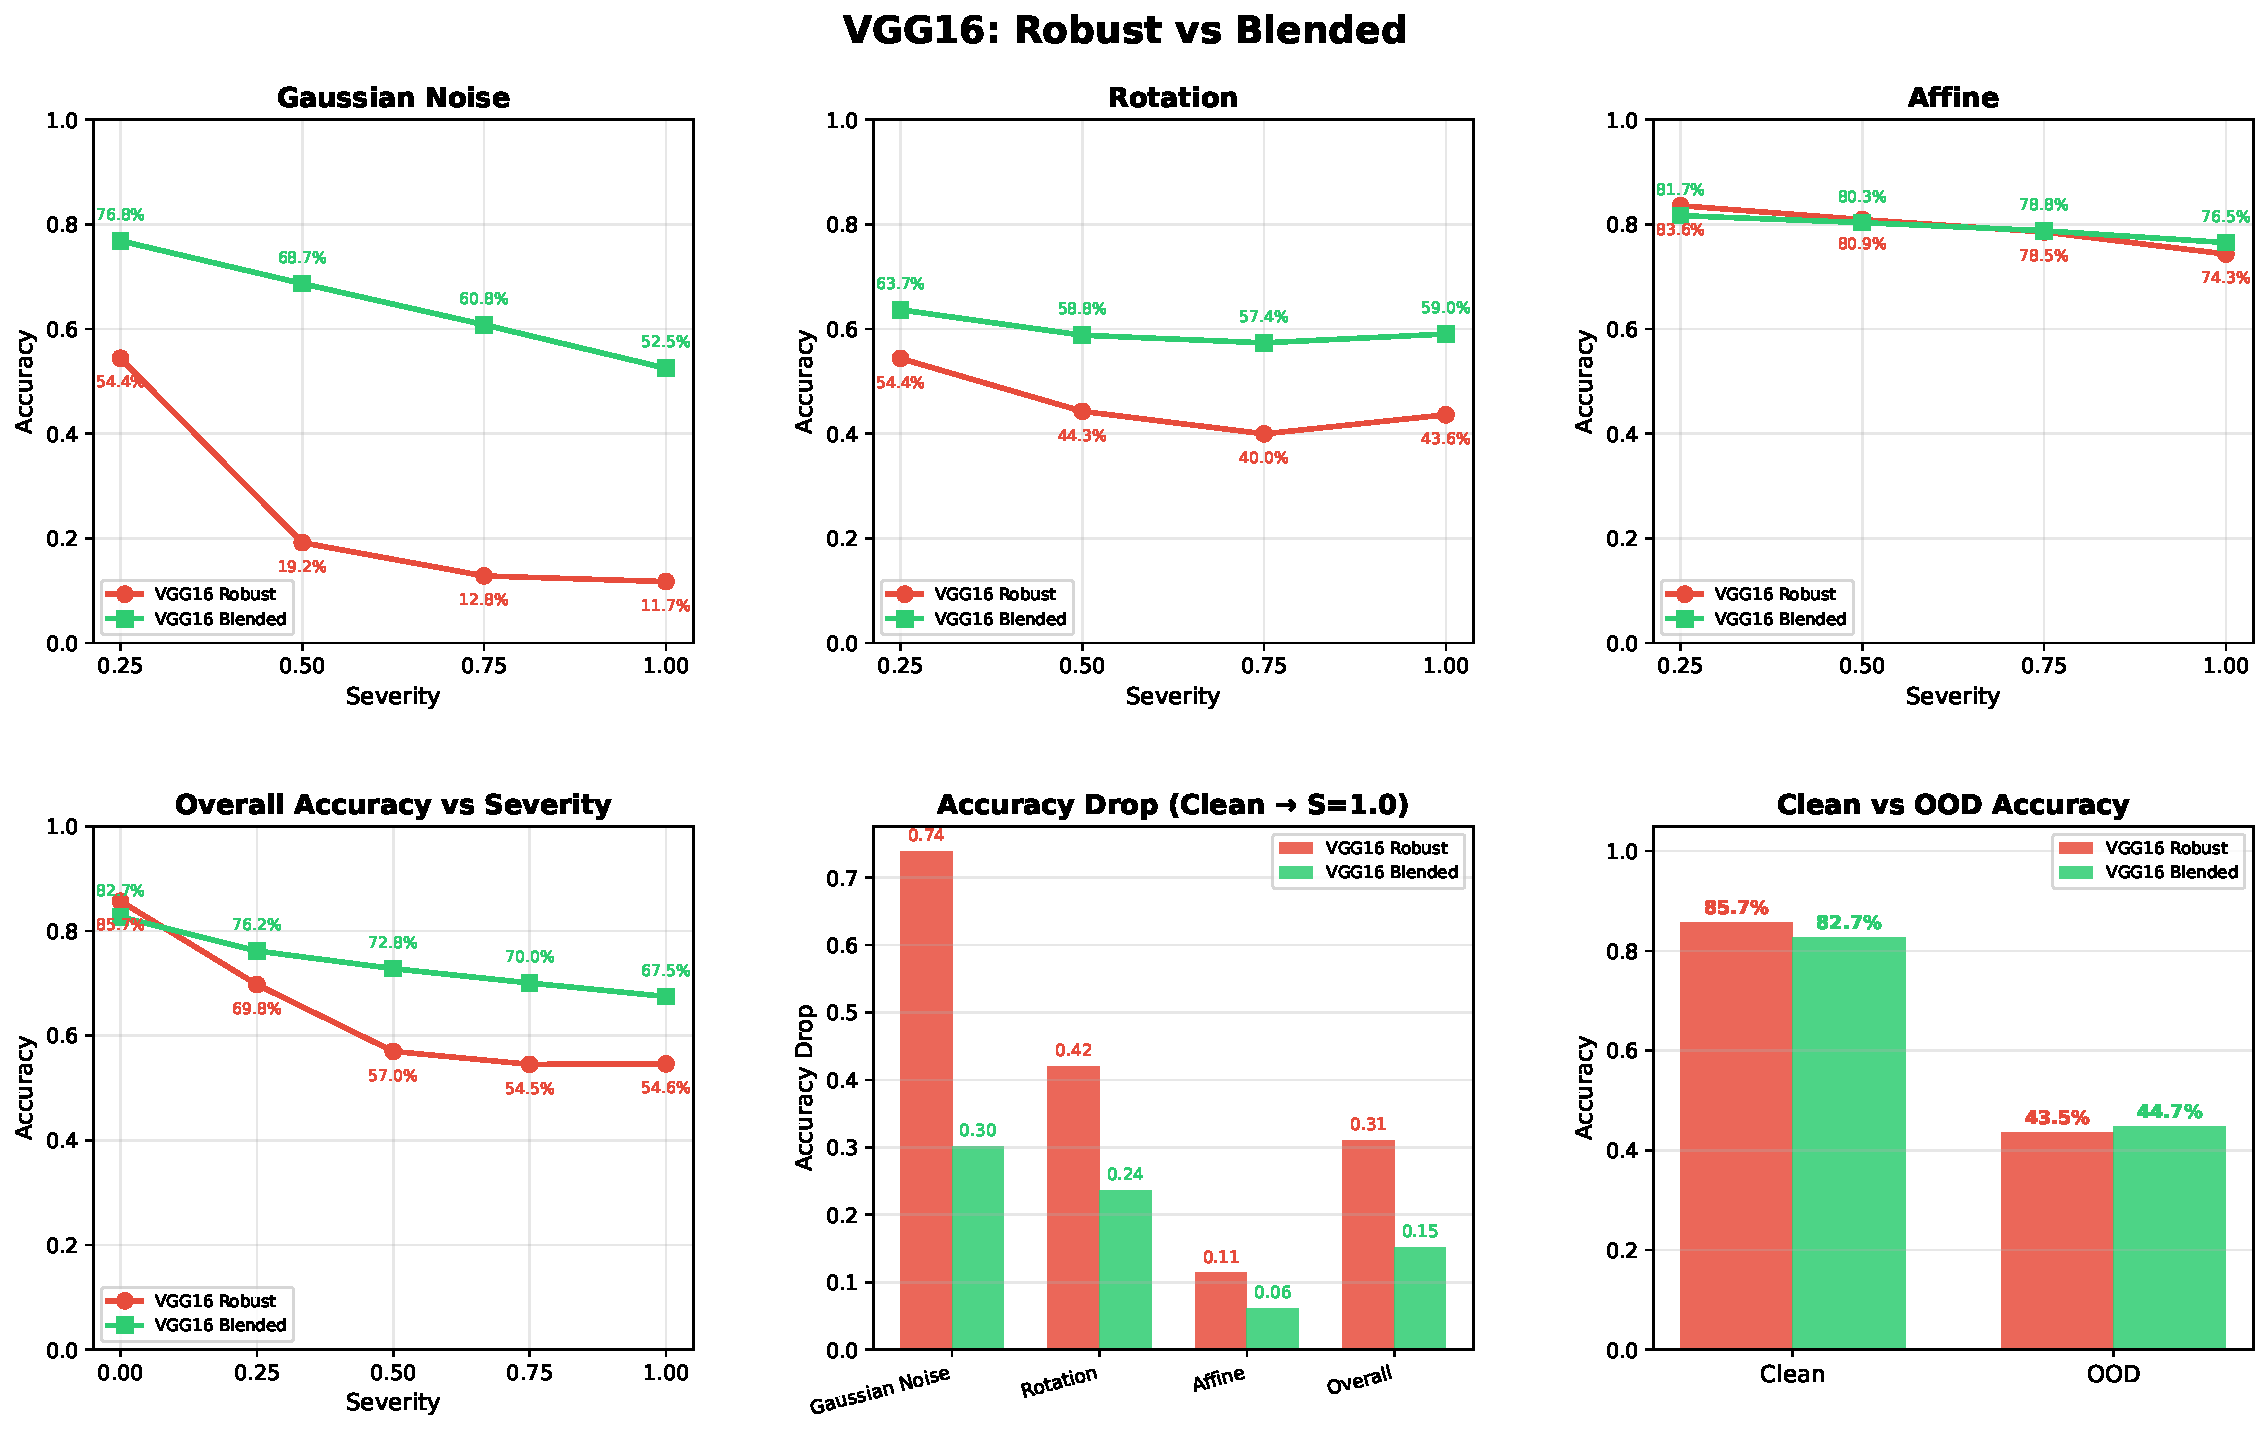
\includegraphics[width=\textwidth]{graphs/pair_vgg16_robust_vs_blended.pdf}
\caption{VGG16: Robust vs Blended across all transforms and OOD.}
\label{fig:vgg16}
\end{figure}

\begin{figure}[H]
\centering
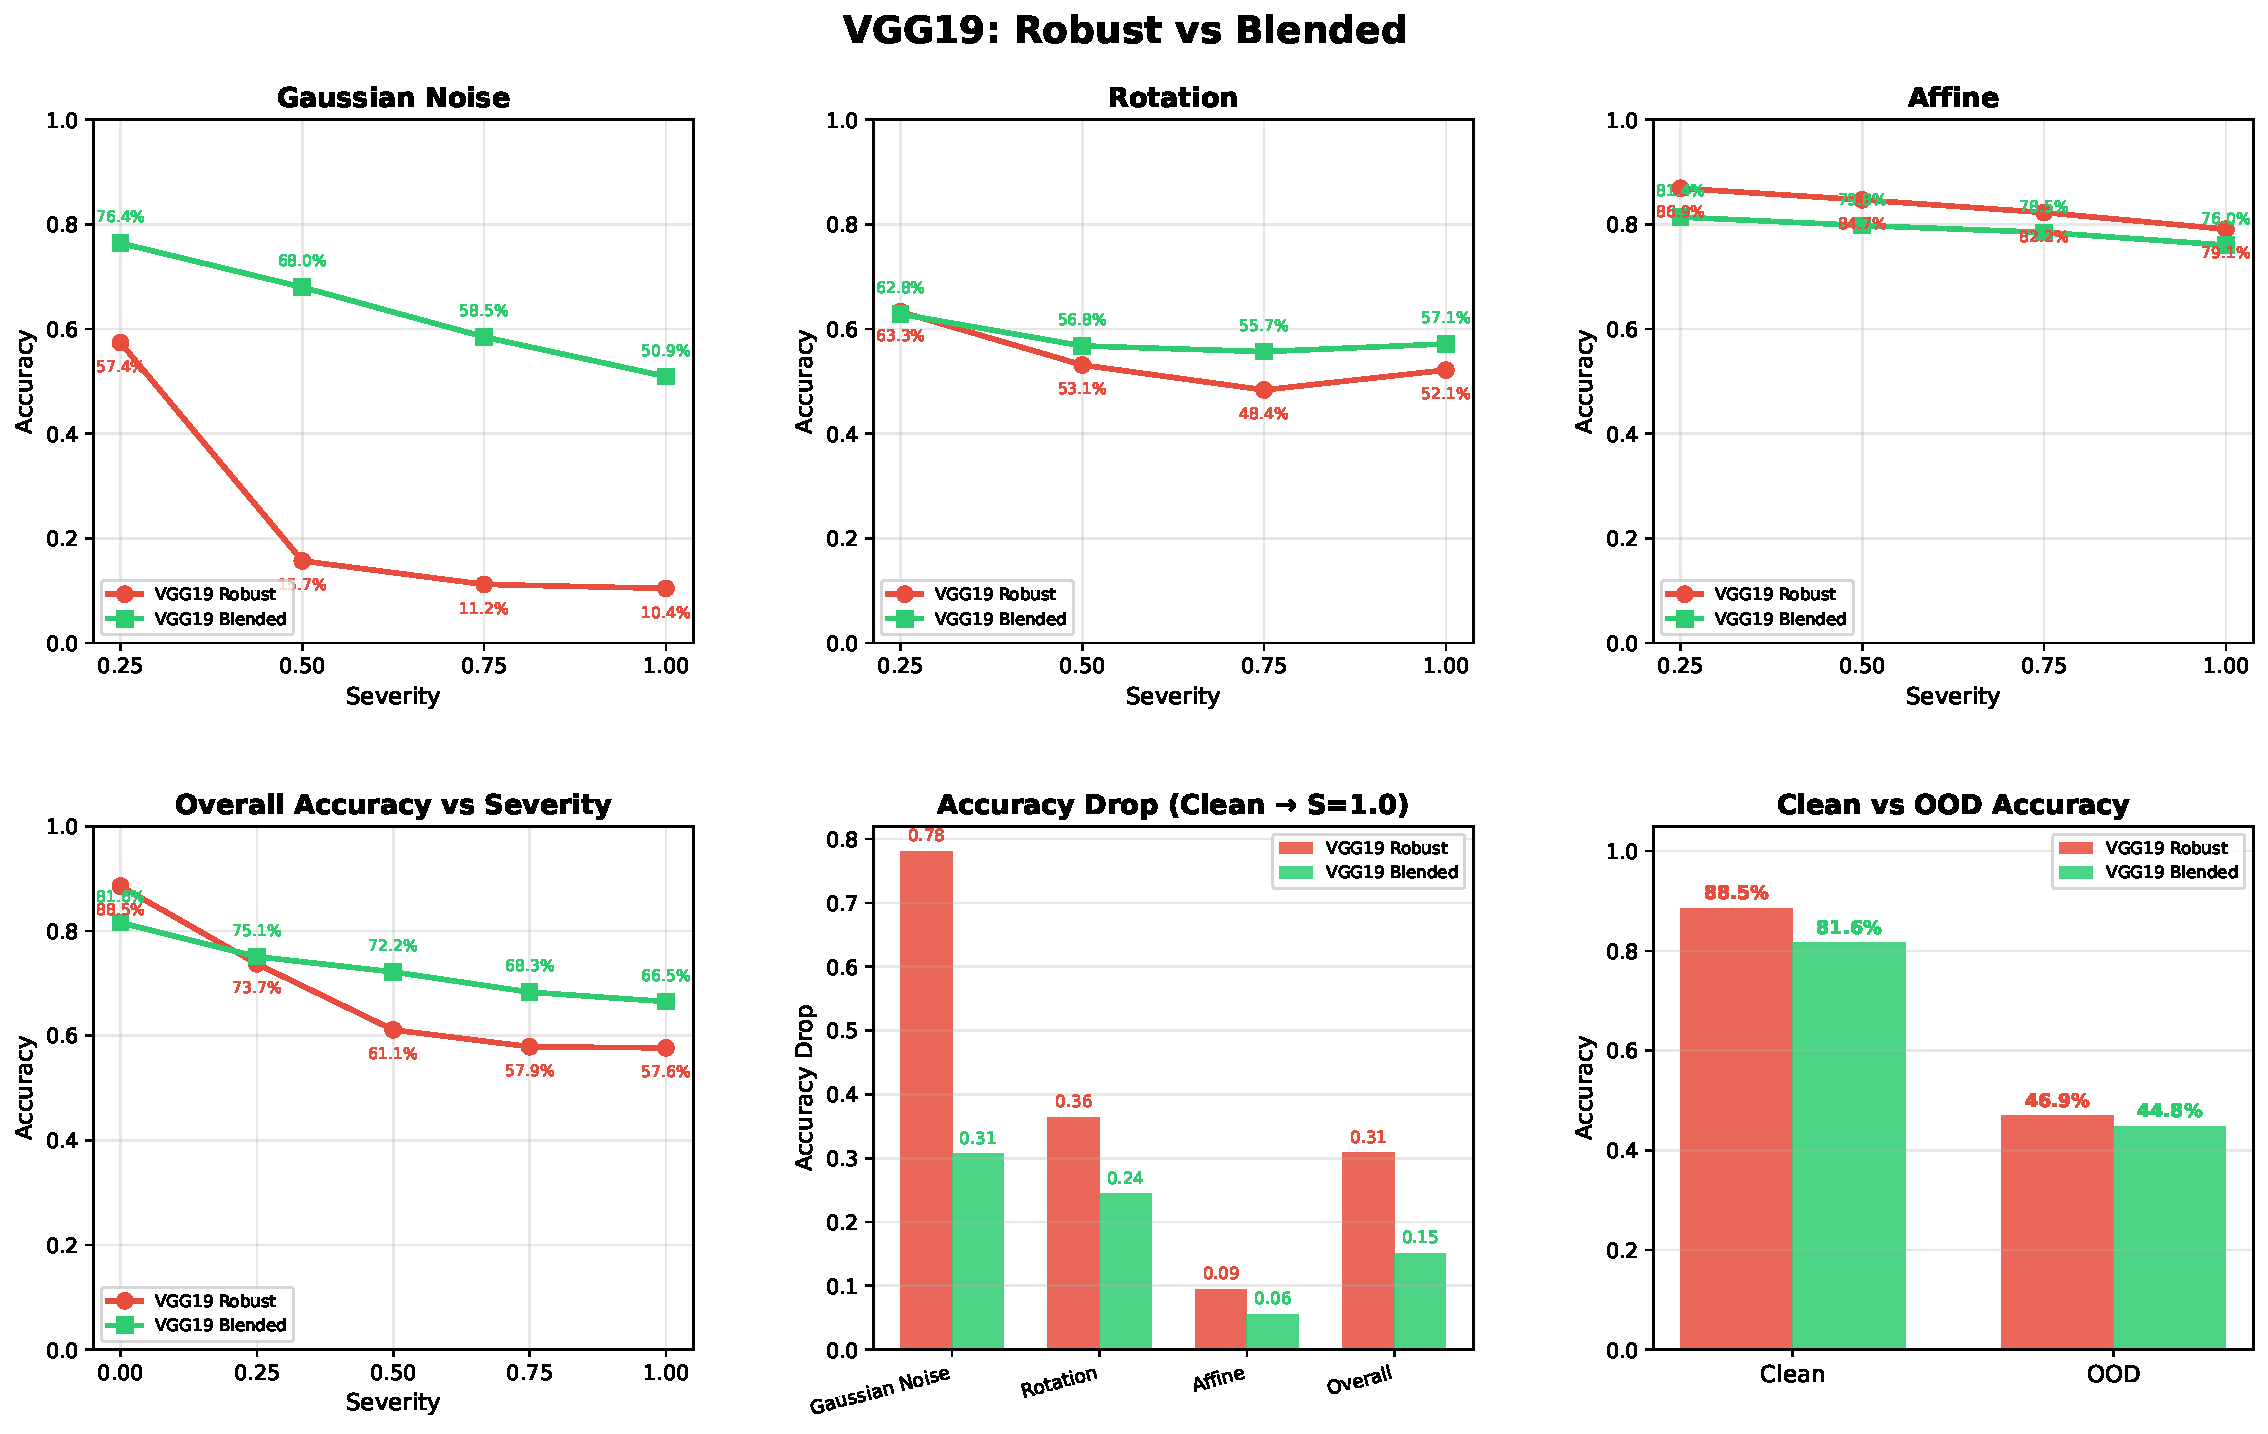
\includegraphics[width=\textwidth]{graphs/pair_vgg19_robust_vs_blended.pdf}
\caption{VGG19: Robust vs Blended across all transforms and OOD.}
\label{fig:vgg19}
\end{figure}

\begin{figure}[H]
\centering
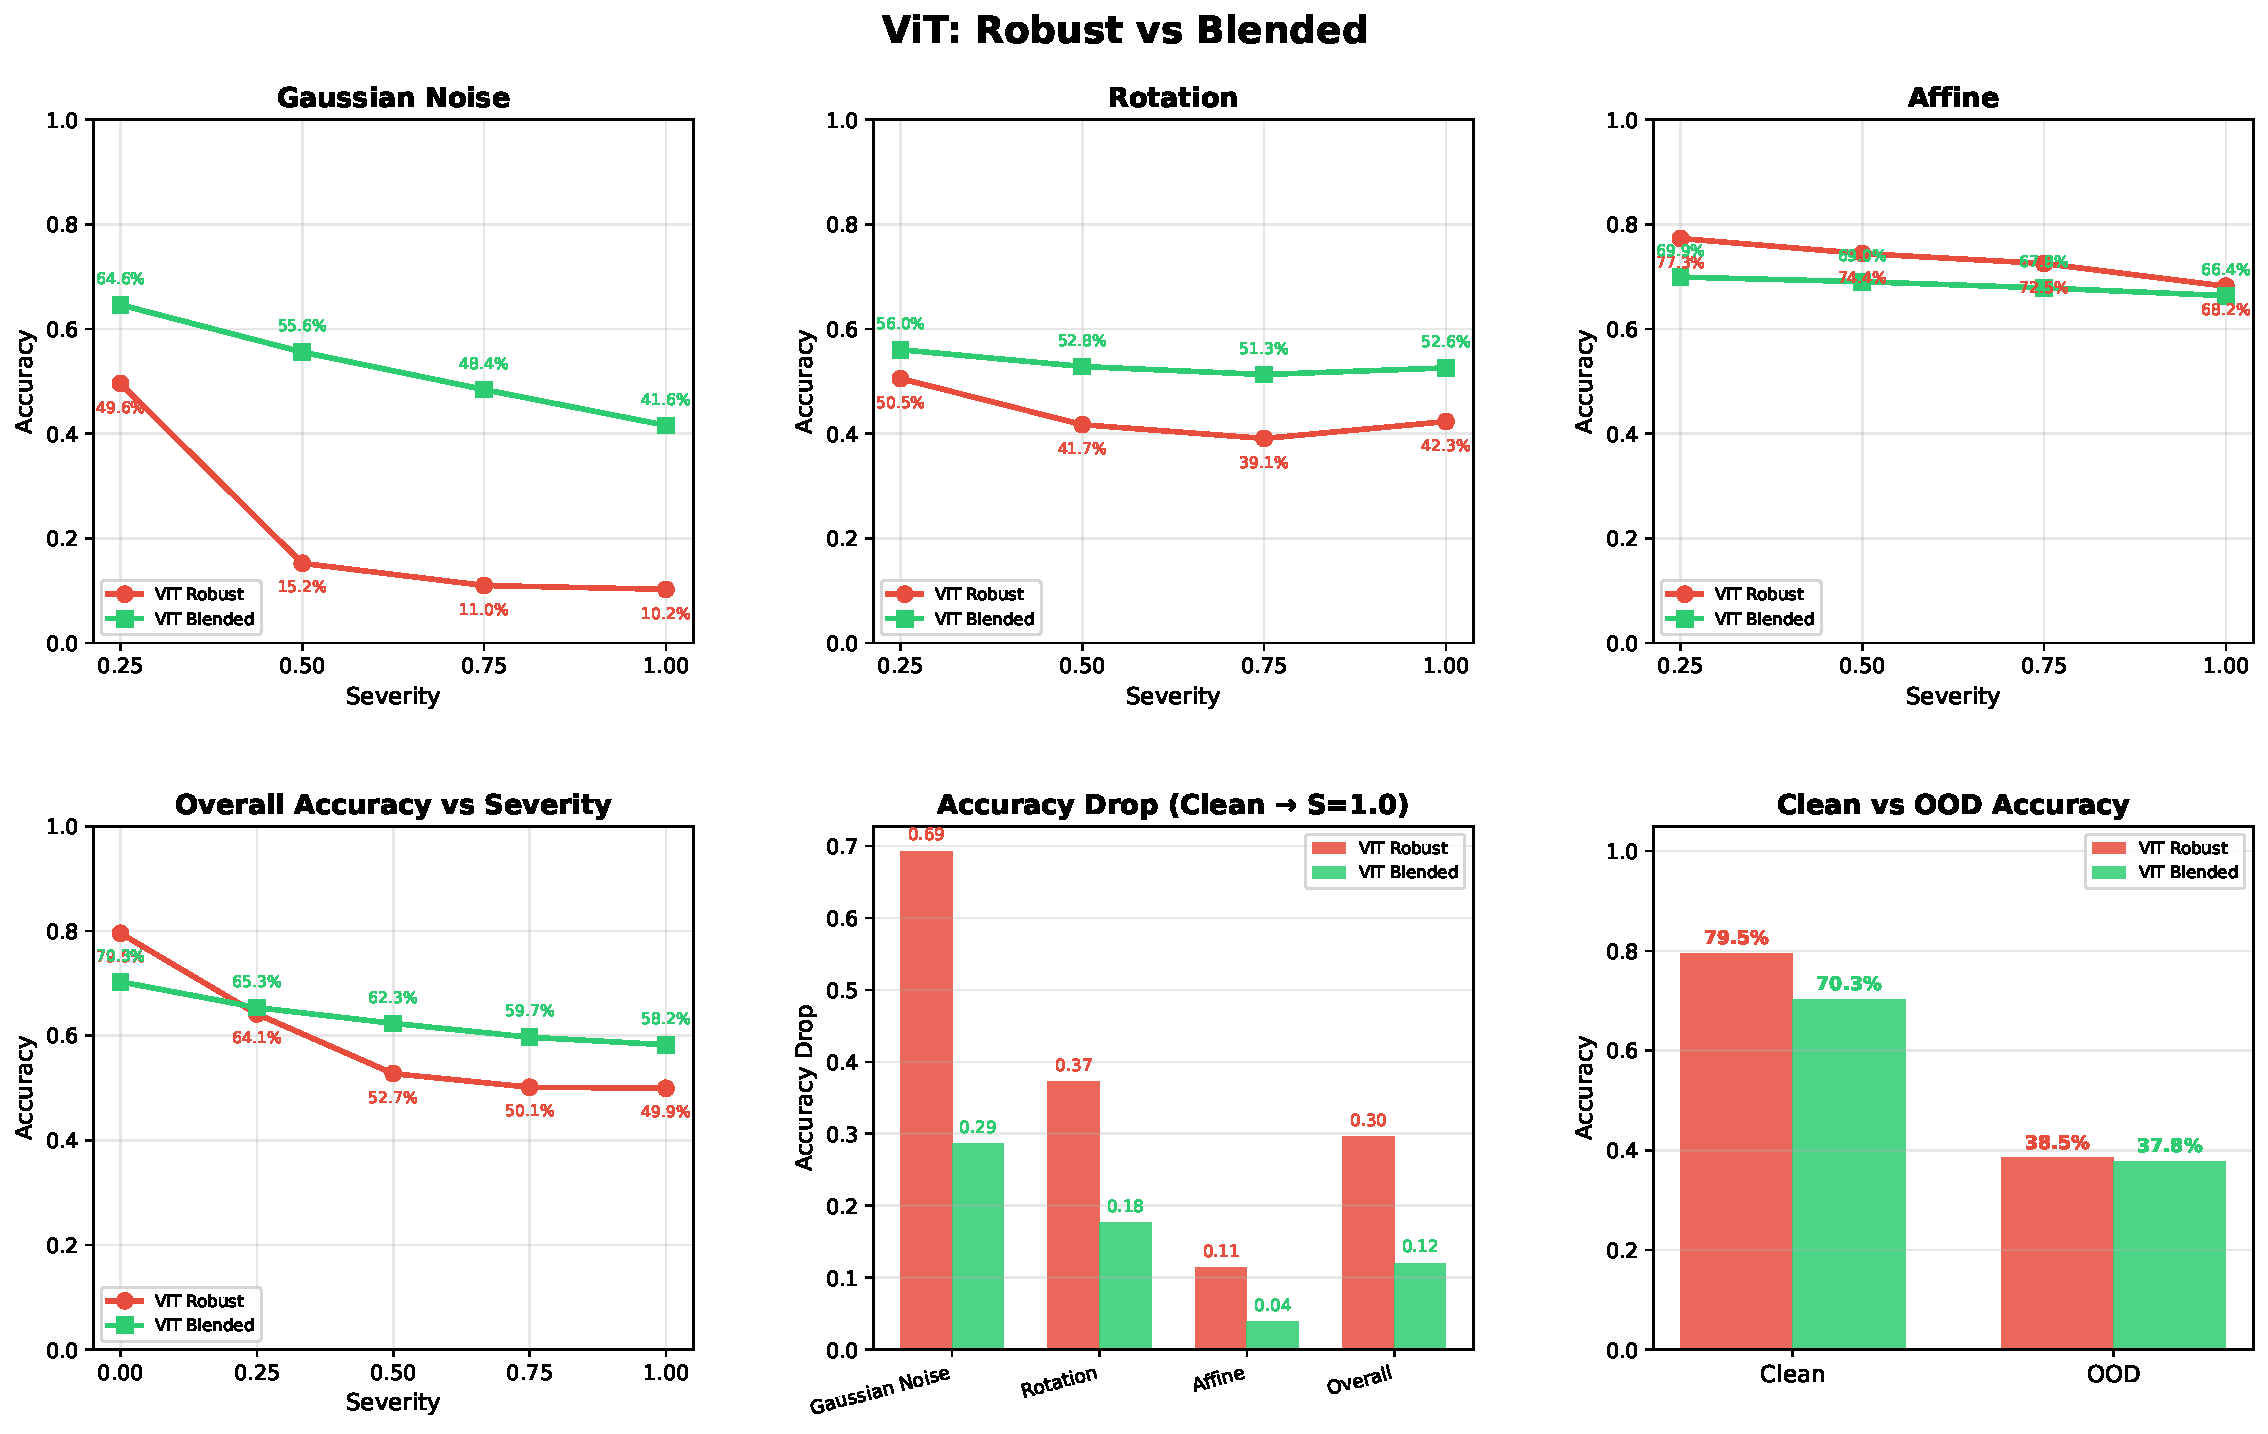
\includegraphics[width=\textwidth]{graphs/pair_vit_robust_vs_blended.pdf}
\caption{Vision Transformer: Robust vs Blended across all transforms and OOD.}
\label{fig:vit}
\end{figure}

%---------------------------------------------------------------------
\section{Analysis}

\subsection{The Auxiliary Loss is Tiny but Transformative}

The transform prediction loss contributes at most $0.01 \cdot \sigma(\mathcal{L}_t) \leq 0.01$ to the total loss multiplier. Despite this negligible direct gradient signal, the auxiliary task forces the backbone to learn features that distinguish corruption from content. This implicit regularization makes the learned representation inherently robust.

\subsection{Gaussian Noise Resilience}

The most dramatic improvement is under Gaussian noise at $s = 1.0$: Robust models collapse to $\sim$10\% (random chance on 10 classes), while Blended models maintain 42--53\%. The transform prediction task teaches the model to recognize noise patterns, effectively learning an implicit denoising mechanism.

\subsection{The Residual Design is Key}

The residual connection $\mathbf{h}_{\text{enhanced}} = \mathbf{h}_{\text{backbone}} + \text{FusionMLP}([\mathbf{h},\, \hat{\mathbf{t}}])$ ensures the transform-aware pathway can only \emph{add} information to the base features. If the fusion module produces unhelpful outputs, the model can learn to zero them out, falling back to the original backbone features. This provides a ``safety net'' that explains why clean accuracy remains competitive.

\subsection{Clean Accuracy Trade-off}

For VGG16/VGG19/ViT, Robust models achieve slightly higher clean accuracy (by 3--9 percentage points). This trade-off is expected: Blended models allocate some representational capacity to transform prediction. However, the robustness gain far outweighs this cost. For ResNet18, the Blended model achieves \emph{higher} clean accuracy (83.1\% vs 66.5\%), suggesting the auxiliary task acts as beneficial regularization for smaller models.

\subsection{OOD Generalization}

On 10 extreme corruptions never seen during training, Blended models match or exceed Robust models in 3 of 4 backbones (ResNet18: 46.6\% vs 34.1\%, VGG16: 44.7\% vs 43.5\%, VGG19: 44.8\% vs 46.9\%). This demonstrates that the transformation-aware features provide genuine generalization, not memorization of training augmentations.

%---------------------------------------------------------------------
\section{Conclusion}

Adding a minimal auxiliary task---predicting which augmentation transform was applied, with an effective loss weight of just 1\%---consistently and substantially improves model robustness across all tested architectures. The key insight is that \emph{knowing what happened to the input} teaches the model to disentangle content from corruption, yielding features that degrade gracefully under both seen and unseen corruptions. This approach requires no additional data, adds minimal architectural overhead (4 linear heads + 1 two-layer MLP), and has negligible computational cost during training.

\end{document}
